\chapter{Work Done So Far}
Sprints One, Two and Three have been completed as of the time of writing.

\section{Sprint One - Translation Lookup}
The sprint began by looking into technologies to translate the word being clicked on. Possibilities considered were online translation services such as \textcite{googletranslate} and \textcite{bingtranslate}, raw datasets such as the \textcite{dictCC} and Dictionary APIs such as the \textcite{oxford} and the \textcite{collins}. 

The technology that would be used in the project would have to:
\begin{itemize}
	\item Be able to translate single words from to English
	\item Provide Lexical information of those words
	\item Be allowed for the content to be hosted and provided through a web interface
	\item Be available for less than \pounds150 total
\end{itemize}

The five technologies cited above were checked against these criteria and the results are show in Table \ref{tbl:comp}

\begin{table}
\centering
\caption[Comparison of Translation Software]{Comparison of various translation solutions to see whether or not they fulfil the criteria of the application. }
\label{tbl:comp}
\begin{tabu} to \textwidth{|X[c]|X[c]|X[c]|X[c]|X[c]|}
\hline
\textbf{Product}        & \textbf{German to English Translations} & \textbf{Lexical Information} & \textbf{Allowed Online} & \textbf{Less Than \pounds150  (total)} \\ \hline
Google Cloud Translate  & Yes                                     & No                           & Yes                     & No                               \\ \hline
Microsoft Translator    & Yes                                     & No                           & Yes                     & No                               \\ \hline
Dict.cc Dataset         & Yes                                     & Yes                          & No                      & Yes                              \\ \hline
Oxford Dictionaries API & Yes                                     & Yes                          & Yes                     & Yes                              \\ \hline
Collins Dictionary API  & Yes                                     & Yes                          & Yes                     & No                               \\ \hline
\end{tabu}
\end{table}

As \textcite{oxford} was the only technology to clear all four criteria, the decision was made to used it for development of the application, however other technologies were used in testing the resulting code.

\textcite{oxford} is a REST API where two calls are required to get the desired information. The first, to the lemmatron, checks that the word is in the dictionary and provides a list of entries of unconjugated words, their lexical categories and grammar information. The second call is to lookup translations of this uncojugated word, this is illustrated in figure \ref{fig:odsf}

\begin{figure}
	\caption{Systems Flow Diagram of the Oxford Dictionaries API}
	\label{fig:odsf}
	\begin{center}
	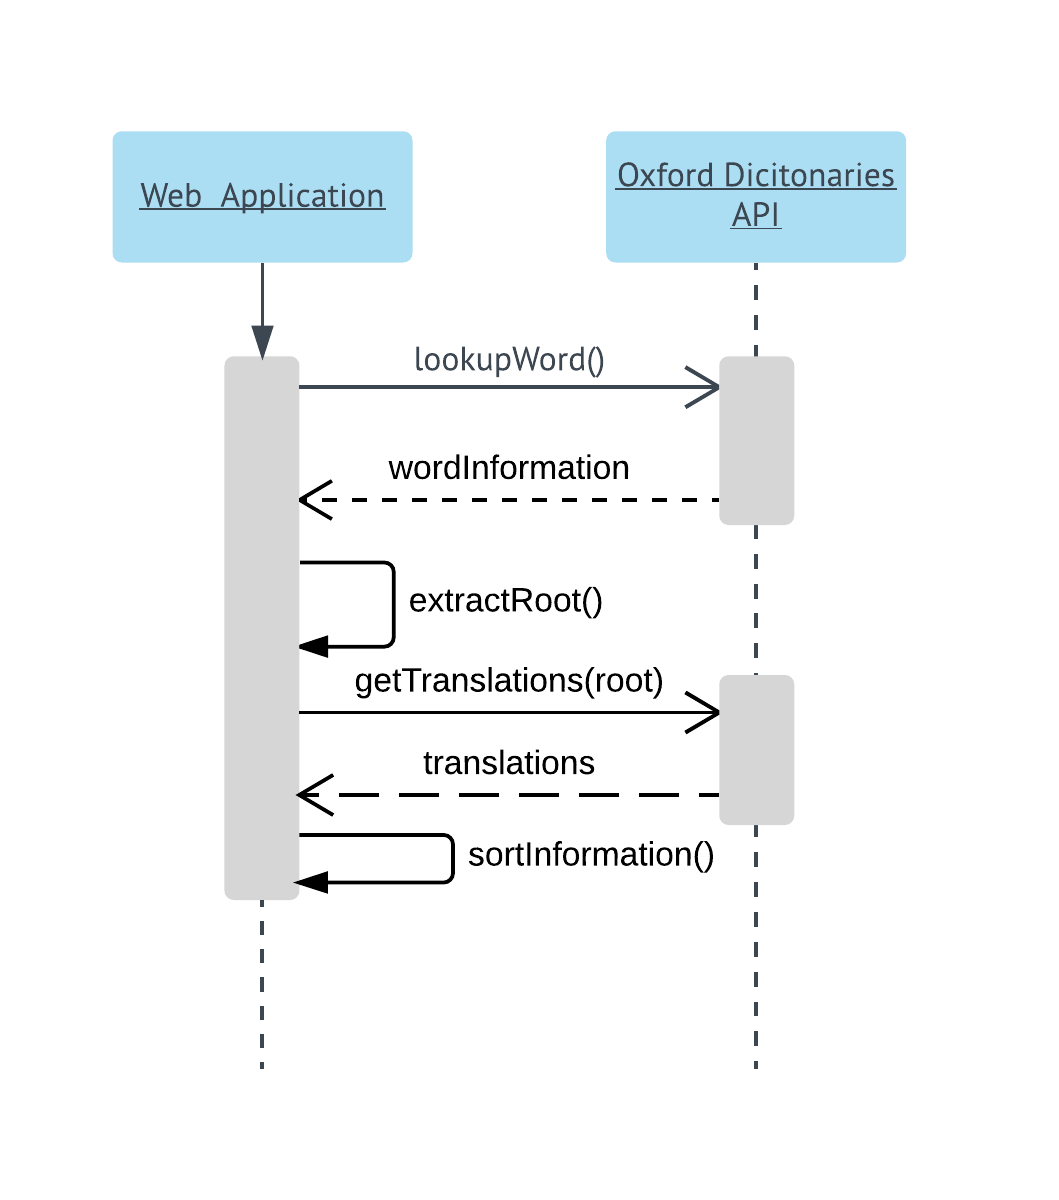
\includegraphics[width=0.7\textwidth]{Graphics/SystemsFlowOxford}
\end{center}
\end{figure}

On the first call, the application takes the first entry provided by the response and extracts the root of the word along with the lexical category and the grammar of the conjugation. Then, on the second call, it compares lexical categories to ensure it's the correct word, before extracting English translations of the root. This information is then passed to a storage class.

Once this part of the application had been written, it was unit tested with a selection of random German words, the unconjugated word, translations and lexical information were compared to results provided by the other technologies and the developer's knowledge. The code passed testing as the results provided were accurate and contained the necessary grammatical information. 

The code for this sprint can be seen in listing \ref{app:dictcode}

\section{Sprint Two - Article Parsing \& Presentation}

A parsing library was used that returns the content of the article as a single string.  As each word would be clicked on individually in the application, a function was written that took this string an returned a two dimensional. The first dimension being paragraphs and the second one being alternating strings of words and punctuation so that each word was individually accessible. This array, was then written to a storage class, along with various bits of meta data that was either extracted by the parsing library or retrieved separately.  

The code for this part of sprint two can be seen in listing \ref{app:parsing}

The second part of this sprint was to enable for these parsed articles to be displayed. For this, a web application was written. This app displayed the parsed article on the left, with a margin on the right left for the gloss content. This view is similar to the wireframe shown in figure \ref{fig:view3}. Each word extracted while parsing was wrapped in a span tag, allowing for easier identification by the AJAX.

The code for this part of the sprint can be seen in listings \ref{app:flask} (web app) and \ref{app:article} (article display template)

The whole sprint was then tested by displaying some articles from the German website "Spiegel Online". The articles displayed nicely and the content of the text was correct, so the sprint passed the tests.

\section{Sprint Three - AJAX}

Sprint three was to connect the now displayed article with the dictionary api, allowing for the translations of a word to appear in the margin, once that word is clicked on. To do this, a function was assigned to the on-click listener of the span tag surrounding each word. When this function was called, a request would be sent to the server containing the word. The word is then be passed to the dictionary code written in sprint one, where the translations and lexical information would be retrieved from \textcite{oxford}. This information is then passed into a template and sent back to the webpage, where the new template is inserted into the margin on the right. 

CSS classes for the various lexical categories were defined to give each lexical category its own colour scheme, and the ability to remove entries was implemented by adding close button in the top right corner of the entry, with the appropriate function. 

The code was then tested using the same articles used in sprint two, making sure that the gloss entries were displayed as expected, and that they were for the right word and the content displayed in them was correct. 

The code for this sprint can be found in listings \ref{app:javascript} (javascript) and \ref{app:dictcss} (css classes)

